\documentclass[10pt]{beamer}

\mode<presentation>
{
  \usetheme[height=1.25cm]{Madrid}
  \setbeamertemplate{navigation symbols}{}
  \setbeamercolor{alerted text}{fg=illini}
}
\graphicspath{{./}{figs/}{/Users/hic/Dropbox/To-process/slides/pics/}{/Users/hic/Dropbox/To-process/slides/pics/feat-det/}{/Users/hic/Dropbox/To-process/slides/3630-08/}{/Users/hic/Dropbox/To-process/slides/8803-09/}{/Users/hic/Dropbox/To-process/slides/8803-12/}{/Users/hic/Dropbox/To-process/slides/8803-08/}}

\usebackgroundtemplate{
\includegraphics[width=\paperwidth,height=\paperheight]{uc-background}}

\usepackage[english]{babel}
\usepackage{epsfig,subfigure,bm}
\usepackage{multimedia}
\usepackage{psfrag}
\usepackage{animate}

% \usefonttheme{metropolis} % default family is serif
%%%%%% Begin of my macros and options

\setbeamertemplate{section in toc shaded}[default][55]
\setbeamertemplate{subsection in toc shaded}[default][55]
\setbeamercolor{block title}{fg=white,bg=illini}
\setbeamercolor{block body}{fg=black,bg=mygrey}

\setbeamercolor{emphprimary}{fg=CBlue}
\setbeamercolor{emphsecondary}{fg=illini}
\setbeamercolor{emphtertiary}{fg=mygreen}
\definecolor{darkForestGreen}{rgb}{.1,1,.1}
\definecolor{veryLightGray}{rgb}{.9,.9,.9}
\definecolor{greenApple}{rgb}{.3,.9,.3}

\setbeamercolor{title}{bg=CBlue}

\usepackage{amsmath,amssymb,amsxtra,amsthm}
\usepackage{algorithm,algorithmic}
\usepackage{natbib}
\usepackage{bibentry}
\usepackage{xspace}
\usepackage{changepage}

\definecolor{myblue}{rgb}{.2,.2,.7}
\definecolor{myred}{rgb}{.7,.2,.2}
\definecolor{mygreen}{rgb}{.2,.7,.2}
\definecolor{mygrey}{rgb}{0.9,0.9,0.9}
\definecolor{CBlue}{cmyk}{1,0.25,0,0}
\definecolor{illini}{rgb}{0.98,0.4,0.05}
\definecolor{black}{cmyk}{0,0,0,1}

\newcommand{\myemph}[1]{{\usebeamercolor[fg]{emphprimary}
    \textbf{#1}}}
\newcommand{\myemphalt}[1]{{\usebeamercolor[fg]{emphsecondary}
    \textbf{#1}}}


\title[Math for Robotics] % (optional, use only with long paper titles)
{CSE276C - Markov Chains}

\author[H.~I. Christensen] % (optional, use only with lots of authors)
{Henrik I.~Christensen}
% - Give the names in the same order as the appear in the paper.  -
% Use the \inst{?} command only if the authors have different
% affiliation.

\AtBeginSection[]
{
   \begin{frame}
       \frametitle{Outline}
       \tableofcontents[currentsection]
   \end{frame}
}

\institute[UCSD] % (optional, but mostly needed)
{
  \begin{minipage}[c]{.2\textwidth}
    
\includegraphics[width=.65\linewidth]{ucsealnew}%
  \end{minipage}%
  \begin{minipage}[c]{.6\textwidth}
    \small
%%    \begin{center}
      Computer Science and Engineering\\
      University of California, San Diego\\
%%    \end{center}

  \end{minipage}
%%  \vspace*{1ex}
}
%% - Use the \inst command only if there are several affiliations.
%% - Keep it simple, no one is interested in your street address.

\bigskip

\date[Dec 2020]% (optional, should be abbreviation of conference name)
{\small%
  December 2020}

\begin{document}

\nobibliography{/Users/hic/Dropbox/bibliography/bib-file.bib}
\bibliographystyle{plain}

\begin{frame}[plain]
  \titlepage
\end{frame}


\begin{frame}
  \frametitle{Introduction}
  \begin{itemize}
  \item How do we model temporal ``discrete'' processes with
    Associated uncertainty?
  \item Lots of examples in robotics
    \begin{itemize}
    \item Executing a plan
    \item Modeling traffic
    \item Receiving packages for logistics
    \end{itemize}
  \item Basic coverage of the underlying theory
  \end{itemize}
\end{frame}

\begin{frame}
  \frametitle{Independent Trials}
  \begin{itemize}
  \item A set of possible outcomes $X_1, X_2, \ldots$ is given
  \item Each outcome has an associated probability $p_k$
  \item The probability of a samples sequence is given by
    \[
      P \{ (X_{j0}, X_{j1}, \ldots, X_{jk}) \} = p_{j0} p_{j1} \cdots p_{jk}
    \]
  \end{itemize}
\end{frame}

\begin{frame}
  \frametitle{Markov Chains -- Introduction}
  \begin{itemize}
  \item The outcome of any trial dependent on the outcode of the
    directly precedings trial only
  \item \myemph{Conditional Probability $p_{jk}$}: given $X_j$ has
    occured at some trial the probability of $X_k$ at the next trial
  \item $a_k$ is the probability of $X_k$ at the initial trial
  \item I.e.:
    \[
      \begin{array}{rcl}
        P\{ ( X_j, X_k) \} &=& a_k p_{jk}\\
        P\{ ( X_j, X_k, X_l) \} &=& a_j p_{jk} p_{kl}\\
        P \{ (X_{j0}, X_{j1}, \ldots, X_{jk}) \} &=& a_{j0} p_{j1} \cdots p_{jk}\\
      \end{array}
    \]
  \end{itemize}
\end{frame}

\begin{frame}
  \frametitle{Example -- Random Walk}
  \begin{itemize}
  \item How would you model a random walk? \pause
  \item Events: $\{ \ldots, -3, -2, -1, 0, 1, 2, 3, \ldots \}$
  \item $p_{ij} = 0$ if $|j-k| > 1$
  \item $p_{ij} = \frac{1}{2} \mbox{ for } |i-j| = 1$
  \end{itemize}
  \centerline{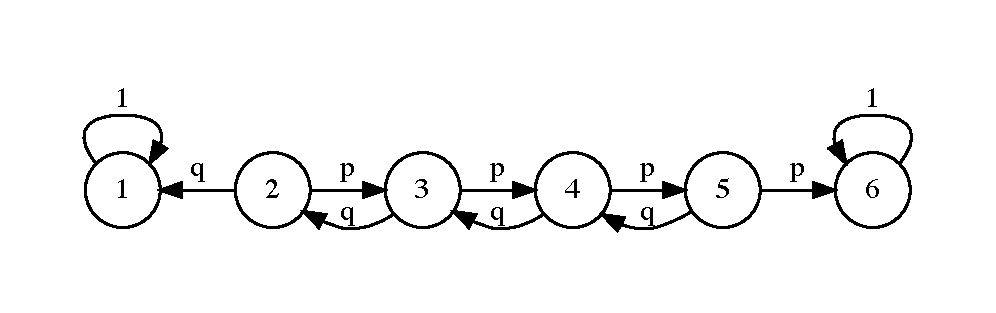
\includegraphics[height=2.5cm]{basic-mc}}
\end{frame}

\begin{frame}
  \frametitle{Formalizing things}
  \begin{itemize}
  \item The chain is in a \myemph{state} $X_t$ at time t.
  \item The \myemph{state space} of a chain is the value X can take
    on, i.e., $S = \{ 1, 2, 3, 4, 5, 6\}$. Let the size of S be N
    (possibly infinite)
  \item A \myemph{trajectory} of a chain is the set of values of X over time, say
    $X_0, X_1, X_2, \ldots$ The trajectory is the ``path'' through a chain.
  \item The \myemph{Markov Property} implies that the future
    state/trajectory only depends upon the current state, i.e.:
    \[
      P(X_{t+1} = s | X_t = s_t, X_{t-1} = s_{t-1}, \ldots, X_0 = s_0) = P(X_{t+1} = s | X_t = s_t)
    \]
  \item A sequence of discrete events random variables can be
    considered a Markov chain if it satisfies the above property
  \end{itemize}
\end{frame}



\end{document}
